% Drawing 142/06-12 -- folder 142, batch 06, archive page 112 (PDF page 113).
% Transcription: Au crayon, trois bandes concentriques qui figurent le revêtement au-dessus de $\Sigma$ ; on y lit les points $Q_1$, $Q_2$, $Q_3$ (marqués d'une croix), $Q^{\omega'}_1$, $Q^{\omega^2}_1$, $Q^{\omega'}_3$, $Q^{\omega}_3$, et, autour de chaque trou $R_i$, les points $R_{i,\omega}$, $R_{i,\omega'}$, $\tilde R_i$, $-\tilde R_i$, $R^\omega_i$, $R^{\omega'}_i$, $-R^\omega_i$, $-R^{\omega'}_i$. Autour de $R_1$ et de $R_2$, à l'encre, de petits quadrilatères de flèches courbes reliant ces points.
% Kind: covering of the sphere drawn as concentric bands, with marked points. Method 2 (schematic redraw from the facsimile). Status: partial.
% Notes: Three concentric pencil bands (the covering over Sigma), drawn as three closed curves; Q_1, Q_2, Q_3 as small crosses; the pencil cross-section joining the bands at Q_1^{omega'} - Q_1^{omega^2} (upper right) and the inked one at Q_3^{omega'} - Q_3^omega (bottom); round the hole R_3 at the top, the section R_3^{omega'}, tilde R_3, R_3^{omega'} above and -tilde R_3, -R_3^{omega'} below, and the small loop R_{3,omega}, R_3, R_{3,omega'}; round R_1 (lower left) and R_2 (lower right) the small oriented circles (R_{1,omega'}, R_{1,omega}; R_{2,omega'}, R_{2,omega}) and the inked quadrilaterals of curved arrows on the points R_1^{omega'}, -R_1^{omega'}, -R_1^omega, R_1^omega (with tilde R_1, -tilde R_1 inside) and tilde R_2^{omega'}, R_2^omega, R_{2,omega}, -R_2^{omega'} (with tilde R_2, -tilde R_2 along the sides); the inked stroke along the outer band at the bottom left. Every side of a quadrilateral ends at its corner points. Still differs: the band outlines are faint and doubled on the page; they are drawn as three smooth closed curves, which is approximate (on the page they are not ellipses); the arrows of the quadrilaterals are drawn schematically (their exact course and every arrowhead are not reproduced, and the doubled sides round R_2 are drawn twice); several small labels are placed only approximately and their indices are a reading. Nothing is struck. Redrawn 2026-11-09 (issue 128): to check again. Question settled by a machine pass on the facsimile, 2026-11-12 (page): the bands are three nested closed curves, as drawn (their exact outline does not change the figure); the labels were compared one by one at 600 dpi and agree with the redraw, except the lower right corner of the quadrilateral round R_2, which reads R_2^omega with a blotted-out second subscript and is now set R_2^omega. Not checked by a reader. 2026-11-13, Claude Opus 5.5, overlay check (issue 147): rasterised from its own coordinates over the 400 dpi colour scan (250 ppi native) on a unit grid; the inked quadrilaterals of curved arrows round R_1 and R_2, the small circles, the cross-sections and the crosses Q_1, Q_2, Q_3 lie near their ink (1 to 2 units; a snap onto the ink did not improve them), so the redraw is unchanged. Not compiled (no TeX in the session). Still differs, as before: the three bands are faint, doubled pencil curves on the page and are drawn as three smooth closed curves, which is approximate (2 to 4 units in places); the arrows of the quadrilaterals are drawn schematically, not each head and course; several small labels are placed approximately.
% Coordinates: 1 unit = 1.6 mm = 1/100 of the crop width (bbox in page fractions: [0.1, 0.08, 0.84, 0.46]).
% Redrawn by Claude (claude-opus-5-5), issue #73, 2026-11-09; not checked by a human; not compiled (no TeX in the session).
% Checked by Claude (claude-opus-5-5) 2026-11-13 (issue #147): overlaid on the 400 dpi colour facsimile; not compiled (no TeX in the session). Not checked by a human. Status: partial.
% Rights: reproduces part of the work -- behind RENDER_TRANSCRIPTS, never published by itself.
\documentclass[tikz,border=3pt]{standalone}
\usepackage{amsmath,amssymb}
\usetikzlibrary{patterns,arrows.meta}
\tikzset{pencil/.style={black!45}, struck/.style={black!35}, mark/.style={circle,draw,inner sep=1.3pt}, pt/.style={circle,fill,inner sep=0.9pt}, opt/.style={circle,draw,fill=white,inner sep=1.1pt}}
\begin{document}
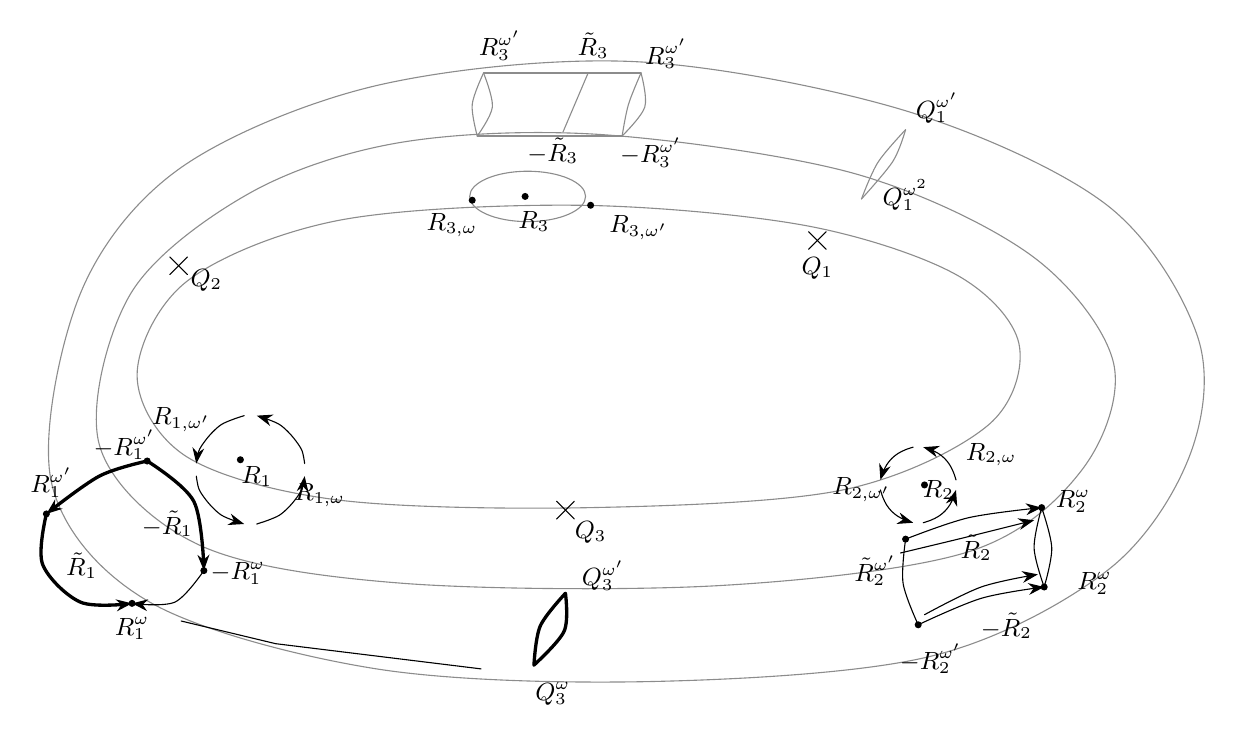
\begin{tikzpicture}[x=1.6mm,y=1.6mm,line cap=round,line join=round,font=\scriptsize]
\draw[pencil] plot[smooth cycle, tension=0.55] coordinates {(48.5,-14.6) (70,-18.5) (86,-26) (93.2,-36.5) (92.5,-46) (86,-55) (72,-61.8) (50,-63.8) (28,-62.8) (10,-57.5) (2.2,-48) (4.5,-33) (12.5,-23) (28,-16.5)};
\draw[pencil] plot[smooth cycle, tension=0.55] coordinates {(46,-20.4) (66,-23.5) (80,-30) (86.5,-38.5) (84,-47) (75,-53.5) (55,-56.2) (30,-56) (14,-53) (6,-45) (8.5,-33) (18,-25) (30,-21)};
\draw[pencil] plot[smooth cycle, tension=0.55] coordinates {(44,-26) (62,-27.6) (74,-31.5) (79,-37) (76.5,-43.5) (65,-48.6) (45,-50) (25,-49.4) (13,-46) (9,-39.5) (13,-32) (25,-27.2)};
\draw (62.3,-28.1) -- (63.7,-29.5);
\draw (62.3,-29.5) -- (63.7,-28.1);
\draw (11.6,-30.1) -- (13,-31.5);
\draw (11.6,-31.5) -- (13,-30.1);
\draw (42.3,-49.5) -- (43.7,-50.9);
\draw (42.3,-50.9) -- (43.7,-49.5);
\draw[pencil] plot[smooth, tension=0.55] coordinates {(70,-20) (69,-22.5) (66.5,-25.5)};
\draw[pencil] plot[smooth, tension=0.55] coordinates {(70,-20) (67.8,-22.6) (66.5,-25.5)};
\draw[very thick] plot[smooth, tension=0.55] coordinates {(43,-56.8) (42.9,-59.8) (40.5,-62.5)};
\draw[very thick] plot[smooth, tension=0.55] coordinates {(43,-56.8) (41,-59.4) (40.5,-62.5)};
\draw[pencil] (36.5,-15.5) -- (44.8,-15.5);
\draw[pencil] (44.8,-15.5) -- (49,-15.5);
\draw[pencil] (36,-20.5) -- (42,-20.5);
\draw[pencil] (42,-20.5) -- (47.5,-20.5);
\draw[pencil] plot[smooth, tension=0.55] coordinates {(36.5,-15.5) (35.6,-18) (36,-20.5)};
\draw[pencil] plot[smooth, tension=0.55] coordinates {(36.5,-15.5) (37.2,-18.2) (36,-20.5)};
\draw[pencil] plot[smooth, tension=0.55] coordinates {(49,-15.5) (48,-18) (47.5,-20.5)};
\draw[pencil] plot[smooth, tension=0.55] coordinates {(49,-15.5) (49.3,-18.2) (47.5,-20.5)};
\draw[pencil] (44.8,-15.5) -- (42.8,-20.2);
\draw[pencil] (40,-25.3) ellipse[x radius=4.6, y radius=2];
\node[pt] at (35.6,-25.6) {};
\node[pt] at (39.8,-25.3) {};
\node[pt] at (45,-26) {};
\draw[-{Stealth[length=2mm]}] plot[smooth, tension=0.55] coordinates {(17.5,-42.7) (16.6,-43) (15.7,-43.4) (15,-44) (14.4,-44.7) (13.9,-45.5) (13.7,-46.5)};
\draw[-{Stealth[length=2mm]}] plot[smooth, tension=0.55] coordinates {(13.7,-47.5) (13.9,-48.5) (14.4,-49.3) (15,-50) (15.7,-50.6) (16.6,-51) (17.5,-51.3)};
\draw[-{Stealth[length=2mm]}] plot[smooth, tension=0.55] coordinates {(18.5,-51.3) (19.4,-51) (20.3,-50.6) (21,-50) (21.6,-49.3) (22.1,-48.5) (22.3,-47.5)};
\draw[-{Stealth[length=2mm]}] plot[smooth, tension=0.55] coordinates {(22.3,-46.5) (22.1,-45.5) (21.6,-44.7) (21,-44) (20.3,-43.4) (19.4,-43) (18.5,-42.7)};
\node[pt] at (17.2,-46.2) {};
\draw[-{Stealth[length=2mm]}] plot[smooth, tension=0.55] coordinates {(70.6,-45.2) (70,-45.4) (69.4,-45.7) (68.9,-46.1) (68.5,-46.6) (68.2,-47.2) (68,-47.8)};
\draw[-{Stealth[length=2mm]}] plot[smooth, tension=0.55] coordinates {(68,-48.6) (68.2,-49.2) (68.5,-49.8) (68.9,-50.3) (69.4,-50.7) (70,-51) (70.6,-51.2)};
\draw[-{Stealth[length=2mm]}] plot[smooth, tension=0.55] coordinates {(71.4,-51.2) (72,-51) (72.6,-50.7) (73.1,-50.3) (73.5,-49.8) (73.8,-49.2) (74,-48.6)};
\draw[-{Stealth[length=2mm]}] plot[smooth, tension=0.55] coordinates {(74,-47.8) (73.8,-47.2) (73.5,-46.6) (73.1,-46.1) (72.6,-45.7) (72,-45.4) (71.4,-45.2)};
\node[pt] at (71.5,-48.2) {};
\node[pt] at (1.8,-50.5) {};
\node[pt] at (9.8,-46.3) {};
\node[pt] at (14.3,-55) {};
\node[pt] at (8.6,-57.6) {};
\node[pt] at (70,-52.5) {};
\node[pt] at (80.8,-50) {};
\node[pt] at (81,-56.3) {};
\node[pt] at (71,-59.3) {};
\draw[very thick,-{Stealth[length=2mm]}] plot[smooth, tension=0.55] coordinates {(9.8,-46.3) (6,-47.5) (1.8,-50.5)};
\draw[very thick,-{Stealth[length=2mm]}] plot[smooth, tension=0.55] coordinates {(9.8,-46.3) (13.5,-49.5) (14.3,-55)};
\draw[-{Stealth[length=2mm]}] plot[smooth, tension=0.55] coordinates {(14.3,-55) (12,-57.5) (8.6,-57.6)};
\draw[very thick,-{Stealth[length=2mm]}] plot[smooth, tension=0.55] coordinates {(1.8,-50.5) (1.5,-54.5) (4.5,-57.5) (8.6,-57.6)};
\draw (12.5,-59) -- (20,-60.8) -- (36.3,-62.8);
\draw[-{Stealth[length=2mm]}] plot[smooth, tension=0.55] coordinates {(70,-52.5) (75,-50.8) (80.8,-50)};
\draw[-{Stealth[length=2mm]}] plot[smooth, tension=0.55] coordinates {(69.6,-53.6) (75,-52.3) (80.2,-51)};
\draw plot[smooth, tension=0.55] coordinates {(80.8,-50) (81.6,-53.2) (81,-56.3)};
\draw plot[smooth, tension=0.55] coordinates {(80.8,-50) (80.2,-53.2) (81,-56.3)};
\draw[-{Stealth[length=2mm]}] plot[smooth, tension=0.55] coordinates {(71,-59.3) (76,-57.2) (81,-56.3)};
\draw[-{Stealth[length=2mm]}] plot[smooth, tension=0.55] coordinates {(71.5,-58.5) (76,-56.3) (80.5,-55.3)};
\draw plot[smooth, tension=0.55] coordinates {(70,-52.5) (69.8,-56) (71,-59.3)};
\node[inner sep=1pt] at (37.8,-13.3) {\small $R_3^{\omega'}$};
\node[inner sep=1pt] at (45.2,-13.3) {\small $\tilde R_3$};
\node[inner sep=1pt] at (51,-14) {\small $R_3^{\omega'}$};
\node[inner sep=1pt] at (42,-21.7) {\small $-\tilde R_3$};
\node[inner sep=1pt] at (49.8,-21.8) {\small $-R_3^{\omega'}$};
\node[inner sep=1pt] at (34,-27.6) {\small $R_{3,\omega}$};
\node[inner sep=1pt] at (40.5,-27.3) {\small $R_3$};
\node[inner sep=1pt] at (48.8,-27.8) {\small $R_{3,\omega'}$};
\node[inner sep=1pt] at (72.5,-18.3) {\small $Q_1^{\omega'}$};
\node[inner sep=1pt] at (70,-25.2) {\small $Q_1^{\omega^2}$};
\node[inner sep=1pt] at (63,-31) {\small $Q_1$};
\node[inner sep=1pt] at (14.5,-32) {\small $Q_2$};
\node[inner sep=1pt] at (45,-52) {\small $Q_3$};
\node[inner sep=1pt] at (46,-55.4) {\small $Q_3^{\omega'}$};
\node[inner sep=1pt] at (42,-64.8) {\small $Q_3^{\omega}$};
\node[inner sep=1pt] at (2.2,-48) {\small $R_1^{\omega'}$};
\node[inner sep=1pt] at (8,-45) {\small $-R_1^{\omega'}$};
\node[inner sep=1pt] at (12.5,-43) {\small $R_{1,\omega'}$};
\node[inner sep=1pt] at (18.5,-47.5) {\small $R_1$};
\node[inner sep=1pt] at (23.5,-49) {\small $R_{1,\omega}$};
\node[inner sep=1pt] at (4.6,-54.6) {\small $\tilde R_1$};
\node[inner sep=1pt] at (11.4,-51.3) {\small $-\tilde R_1$};
\node[inner sep=1pt] at (17,-55.2) {\small $-R_1^{\omega}$};
\node[inner sep=1pt] at (8.6,-59.6) {\small $R_1^{\omega}$};
\node[inner sep=1pt] at (66.5,-48.6) {\small $R_{2,\omega'}$};
\node[inner sep=1pt] at (72.6,-48.6) {\small $R_2$};
\node[inner sep=1pt] at (76.8,-45.8) {\small $R_{2,\omega}$};
\node[inner sep=1pt] at (67.6,-55) {\small $\tilde R_2^{\omega'}$};
\node[inner sep=1pt] at (75.6,-53.2) {\small $\tilde R_2$};
\node[inner sep=1pt] at (83.3,-49.5) {\small $R_2^{\omega}$};
\node[inner sep=1pt] at (85,-56) {\small $R_2^{\omega}$};
\node[inner sep=1pt] at (72,-62) {\small $-R_2^{\omega'}$};
\node[inner sep=1pt] at (78,-59.4) {\small $-\tilde R_2$};
\end{tikzpicture}
\end{document}
